

\documentclass[journal]{IEEEtran}

\usepackage{cite}
\usepackage{amsmath}
\interdisplaylinepenalty=2500
\usepackage{algorithm}
\usepackage[noend]{algpseudocode}
\usepackage{array}
\usepackage{graphicx}
\usepackage{float}

% correct bad hyphenation here
\hyphenation{op-tical net-works semi-conduc-tor}


\begin{document}
\title{Camera calibration using OpenCV}

\author{Wilbert~Pumacay,~\textit{Catholic University San Pablo},~wilbert.pumacay@ucsp.edu.pe\\
        Gerson~Vizcarra,~\textit{Catholic University San Pablo},~gerson.vizcarra@ucsp.edu.pe}

% make the title area
\maketitle

\begin{abstract}
Camera calibration is an important step in several applications, like augmented reality. To do calibration properly using current calibration methods we need to get features we can related in both 2D camera space and 3D world space to estimate the camera parameters that give this mapping. In this context, the use of grid patterns help by giving us the features we need, being the components in the pattern which we must detect in every frame in video.
\\
\\
In this paper we use Zhang \cite{CameraCalibration1} camera calibration technique implemented by OpenCV, and compare results using feature extraction of chessboard corners, symmetric/asymmetric circle grids, and concentric circle grid patterns, the first two, using funnctions implemented in OpenCV and the third one using our algorithm.
\end{abstract}

\begin{IEEEkeywords}
Camera calibration, calibration pattern, circle grid, image processing.
\end{IEEEkeywords}


\section{Introduction}

\IEEEPARstart{T}{he} camera calibration problem consists of finding 11 parameters that describe the mapping between 2D camera space and 3D world space. Six parameters, called extrinsic, come from an homogeneous transform, giving 6 parameters ( rotation and translation around the axes ). The other 5 parameters, called intrinsic, define some internal properties of the camera. This can be expressed in the following transformation equation :

\begin{equation}
  \begin{bmatrix}
    \mu \\
    \nu \\
      1 
  \end{bmatrix} = 
  \begin{bmatrix}
    \alpha & \gamma & \mu_{0} \\
       0   & \beta  & \nu_{0} \\
       0   &    0   &    1
  \end{bmatrix} 
  \begin{bmatrix}
    r_{x_{1}} & r_{y_{1}} & r_{z_{1}} & t_{x}\\
    r_{x_{2}} & r_{y_{2}} & r_{z_{2}} & t_{y}\\
    r_{x_{3}} & r_{y_{3}} & r_{z_{3}} & t_{z}
  \end{bmatrix} 
  \begin{bmatrix}
    x \\
    y \\
    z \\
    1
  \end{bmatrix}
%
\end{equation}

In this equation we can detail each of the variables: $x,y,z$ are original coordinates of an object, $r_{ij}$ and $t_{ij}$ means the rotation and translation values respectively in the model matrix, $\alpha$ and $\beta$ represents the focal length in x and y axis respectively, $\mu_0$ and $\nu_0$ are the coordinates x and y at the optical center.
\\
\\
To find these parameters, camera calibration methods make use of correspondences between 2D and 3D spaces in order to fit the parameters that best describe this mapping. We achieve this by minimizing the following function:

\begin{equation}
  \sum^{m}_{i} \sum^{n}_{j} \Vert TP^{ij}_{3D} - P^{ij}_{2D} \Vert^{2}
\end{equation}

Where we are trying to minimize the difference between the expected projection and the actual projection over some set of features. The key idea is that supplying sufficient features that have a correct mapping, we can get the 11 parameters needed that minimize this function. So, a key part is the detection of these features.
\\
\\
In equation $2$ we are looping through a set of features $n$ that are found in each frame of a video of $m$ frames, so, we basically need to detect some feature points in each frame of video, which is what we focus in this paper.

\section{About the method}
To compare results of feature extraction, we implemented the following pipeline.

\begin{figure}[H]
\centering
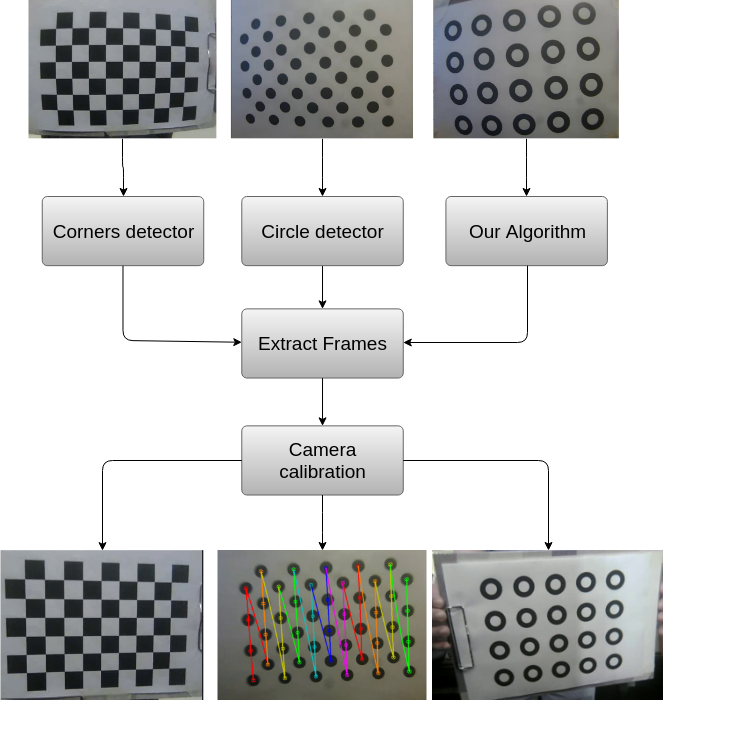
\includegraphics[width=2.5in]{_img/img_report3_pipeline.png}
\caption{Comparison pipeline.}
\end{figure}

\subsection{ Pattern recognition }
We used three principal patterns to calibrate the camera with OpenCV calibration: Chessboard pattern, Circle symmetric/asymmetric pattern and circle concentric pattern. 
\\
\\
In the first two patterns we applied OpenCV implemented functions, and in the third one we used our own algorithm to recognize centers of the circles. In chessboard pattern we have to recognize corners and save their position. In circle pattern we have to detect / recognize circles and save the position of their centers, this pattern has two variations: Symmetric and Asymmetric, both have same purpose. Finally, in circle concentric pattern, similarly to circle pattern, has the main objective to save centers of circles but, with given more circles we can use this to correct the error between both of them.

\subsection{ Our approach in recognition }
We used similar approach to recognize the pattern of previous work \cite{PreviousWork}, with a few modifications:\\
\\
\begin{itemize}
\item We corrected the pattern tracking when it rotates more than 90º degrees.
\item We changed the Region of interest when the program loss the pattern, instead of try to predict position we use all frame to search the pattern.
\item We added a change to pattern to find the orientation, this helps in case when program loss feature points, and when it finds it again, the orientation changes in some cases.
\end{itemize}

%% TODO: Gerson
\begin{algorithm}
\caption{Pattern recognition}
\begin{algorithmic}[1]
\State $\textit{Set up pattern}$
\State $\textit{Set up thresholding parameters}$
\State $mask   = \textit{rgb2gray}( inputImage )$
\State $mask   = \textit{AdaptiveThreshold}(mask, blockSize)$
\State $axis_x   = \textit{Scharr}(masked, 1, 0)$
\State $axis_x   = \textit{Abs}(axis_x)$
\State $axis_y   = \textit{Scharr}(masked, 0, 1)$
\State $axis_y   = \textit{Abs}(axis_y)$
\State $edgesImage   = \textit{Add}(axis_x, axis_y)$ 
\State $\textit{Set up detector parameters}$
\State $\textit{SimpleBlobDetector}(params)$
\State $keypoints   = \textit{detect}(mask)$ 
\State $midPt   = \textit{avg}(keypoints)$
\State $newKeypts[corners] = farthest(keypoints, midPt)$
\State $newKeypts[bord] = near(newKeypts[corners], keypoints)$
\State $newKeypts[rest] = near(newKeypts[bord], keypoints)$
\State $Start tracking$
\State $If pattern is lost: Search again in frame$\\
\Return $newKeypts$
\end{algorithmic}
\end{algorithm}

The pipeline of patter detection and tracking works as follows:

\begin{figure}[H]
\centering
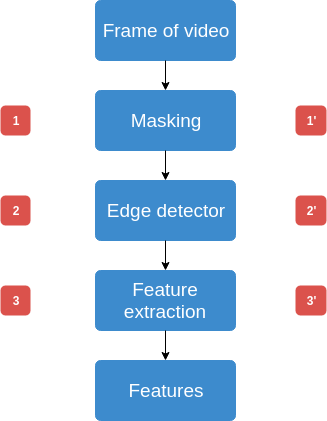
\includegraphics[width=2.5in]{_img/algorithm_overview.png}
\caption{Pipeline of previous work.}
\end{figure}


\section{Results}
%todo wilbert

\section{Conclusions and Future improvements}
%todo wilbert

\IEEEtriggeratref{8}

% references section
\begin{thebibliography}{1}

\bibitem{OpenCV}
  Bradski, G. \\
  \textit{OpenCV library.} - 2000
\\
\bibitem{CameraCalibration1}
  Zhengyou Zhang \\
  \textit{A Flexible New Technique for Camera Calibration.} - 2000
\\
\bibitem{IntegralImageThresholding}
  Derek Bradley, Gerhard Roth \\
  \textit{Adaptive Thresholding Using the Integral Image.} - 2011
\\
\bibitem{PreviousWork}
  Wilbert Pumacay, Gerson Vizcarra\\
  ·\textit{Detection and tracking of circle grid patterns for camera calibration} - 2018

\end{thebibliography}


\end{document}

